\documentclass{article}
\usepackage[T1]{fontenc}
\usepackage[utf8]{inputenc}
\usepackage[portuguese]{babel}
\usepackage[vmargin=3cm]{geometry}
\usepackage{tikzpagenodes}
\usepackage{lipsum}
\usepackage{xcolor}
\usepackage{hyperref}
\usepackage{amsmath}
\usepackage{amssymb}
\usepackage{background}
\usepackage{titlesec}
\usepackage[nodisplayskipstretch]{setspace}
\usepackage{hyphenat}
\usepackage{float}
\usepackage{graphicx}
\hyphenation{mate-mática recu-perar}

\titlespacing{\section}{0em}{-0.5em}{0em}
\titlespacing{\subsection}{0pc}{0em}{0pc}
\titlespacing{\subsubsection}{0pc}{0.33em}{0pc}
\titlespacing{\paragraph}{0em}{0.5em}{0em}
\setlength{\parindent}{2em}
\setlength{\parskip}{1em}
\linespread{1}

\renewcommand{\baselinestretch}{1.0}

\renewcommand\bf[1]{\textbf{#1}}
\renewcommand\it[1]{\textit{#1}}

\newcommand\ov[1]{\overline{#1}}
\newcommand{\vect}[1]{\mathbf{#1}}
\newcommand{\vn}{\varnothing}

\newenvironment{nscenter}
 {\parskip=1.25em\par\nopagebreak\centering}
 {\par\noindent\ignorespacesafterend}

\makeatletter
\def\mcolor#1#{\@mcolor{#1}}
\def\@mcolor#1#2#3{%
  \protect\leavevmode
  \begingroup
    \color#1{#2}#3%
  \endgroup
}
\makeatother
\definecolor{notepadrule}{RGB}{217,244,244}

\backgroundsetup{
contents={%
  \begin{tikzpicture}
    \foreach \fila in {0,...,52}
    {
      \draw [line width=1pt,color=notepadrule]
      (current page.west|-0,-\fila*12pt) -- ++(\paperwidth,0);
    }
    \draw[overlay,red!70!black,line width=1pt]
      ([xshift=-1pt]current page text area.west|-current page.north) --
      ([xshift=-1pt]current page text area.west|-current page.south);
  \end{tikzpicture}%
},
scale=1,
angle=0,
opacity=1
}

\begin{document}

\setlength{\abovedisplayskip}{12pt}
\setlength{\belowdisplayskip}{0.75em}
\setlength{\abovedisplayshortskip}{0pt}
\setlength{\belowdisplayshortskip}{0pt}
% \setlength{\baselineskip}{12pt}
\setlength{\jot}{1pt}

\section*{Lista 2 - Processos Estocásticos}
Davi de Alencar Mendes (16/0026415) \url{dmendes@aluno.unb.br}
\section*{Problema 1}
(Adaptado de [2]) Num sistema de comunicação digital, um bit 0 ou 1 é transmitido com
probabilidade respectivamente igual a $P_0$ ou $P_1$. Devido à presença de ruído no canal, um
0 transmitido pode ser recebido como 1 com probabilidade $\beta$ e um 1 transmitido pode ser
recebido como 0 também com probabilidade $\beta$. Considere agora que foi recebido um bit
interpretado como 1. Qual a probabilidade de que o bit transmitido tenha de fato sido 1?
\\
A probabilidade procurada é $P(T_1|R_1)$ para resolução. Sabendo que:
\begin{align*}
    P(T_0) &= P_0 & P(R_1|T_0) = \beta \\
    P(T_1) &= P_1 & P(R_1|T_1) = \beta \\
    \\
    P(T_1|R_1) &= \frac{P(R_1|T_1)P(T_1)}{P(R_1)} \\
    P(R_1) &= \frac{P(R_1|T_1)P(T_0)}{\beta P_0} + \frac{P(R_1|T_1)P(T_1)}{(1-\beta)P_1} \\
    P(T_1|R_1) &= \frac{(1-\beta)P_1}{\beta P_0 + (1-\beta)P_1} \\[-0.5em]
.\end{align*}

\section*{Problema 2}
Considere que, em um sistema de comunicação digital, $N$ bits são transmitidos em sequência, sendo
cada bit independente dos demais. A probabilidade de que um bit seja recebido corretamente no
receptor é $p$. Acerca desta situação, responda os itens seguintes.

\paragraph*{A.} Deduza a expresão para a probabilidade de que exatamente $(1 \le k \le N)$ bits
sejam recebidos corretamente. \textit{Trata-se da fórmula da probabilidade em uma distribuição
binomial.}

Espaço Amostral: $S = \{(0,0,\ldots,0),(0,0,\ldots,1),\ldots,(0,0,\ldots,1,1),\ldots,(1,1,\ldots,1),\ldots\}$

Cada subconjunto contém $N_P$ elementos. Temos que a cardinalidade de $S$ é: $|S| = 2^{N_P}$
\begin{align*}
    P(I^n_C) &= p \qquad I^n_C \rightarrow \text{bit $n$ é uma transmissão correta} \\
    I^n_0 &= \{(0,0_n,\ldots,0),(0,0_n,\ldots,1),\ldots,(0,0_n,\ldots,1,1),\ldots,(1,0_n,\ldots,1),\ldots\} \\\\
    P(E^{1,2,\ldots,k}_0) &= \; ? \text{ bits } 1,2,3,\ldots,k \text{ com transmissão correta} \\
    E^{1,2,\ldots,k}_0 &= \{0_1,0_2,\ldots,0_k,1_1,1_2,\ldots,1_{N-k}\} \\
    E^{1,2,\ldots,k}_0 &= I_0^1 \cap I_0^2 \cap I_0^3 \ldots \cap I_0^k \cap \ov{I_0^{k+1}} \cap \ov{I_0^{k+2}} \cap \ov{I_0^{N}} \\
    P(E^{1,2,\ldots,k}_0) &= P(I_0^1) \cdot P(I_0^2) \cdot P(I_0^k) \cdot P(\ov{I_0^{k+1}}) \cdot
    P(\ov{I_0^{k+2}}) \cdot P(\ov{I_0^N)} \\
    P(E^{1,2,\ldots,k}_0) &= \underbrace{p \cdot p \ldots \cdot p}_{k} \cdot \underbrace{(1-p)
    \cdot (1-p) \ldots (1-p)}_{N-k} \\
    P(E^{1,2,\ldots,k}_0) &= p^k \cdot (1-p)^{N-k}
\end{align*}

Agora, precisamos generalizar o resultado para o caso de $k$ indivíduos quaisquer, não só os $k$
primeiros. Como existem ${N \choose k}$ possibilidades de extrair $k$ pessoas a partir do grupo de
$N_P$ pessoas, e como os conjuntos $E^{\ldots}$ são disjuntos:

$P(\{k\}) = {N \choose k} p^k (1-p)^{N-k}$, sendo $k$ a união de todos os $E^{(\ldots)}_C$.

\paragraph*{B.} Calcule o valor esperado do número de recepções corretas, dentre as $N$
transmissões.
\begin{align*}
    \mathbb{E}[X] = \int_{-\infty}^{\infty} x f_X(x)dx = \sum_{k=0}^{N} k {N \choose k} p^{k} (1-p)^{N-k}
\end{align*}

Expandindo o primeiro termo vemos que iguala-se a zero e é obtido:
\begin{align*}
    \mathbb{E}[X] &= \sum_{k=1}^{N} \frac{N!}{(k-1)!(N-k)!} p^{k} (1-p)^{N-k} \\
    \text{Fazendo } j &= k-1, \;\; M = N-1 \\
    \mathbb{E}[X] &= \sum_{j=0}^{M} \frac{(M+1)!}{j!(M-j)!} p^{j+1} (1-p)^{M-j} \\
    \mathbb{E}[X] &= (M+1)p \cdot \sum_{j=0}^{M} \frac{M!}{j!(M-j)!} p^{j} (1-p)^{M-j} \\
    \mathbb{E}[X] &= Np \cdot 1
\end{align*}

\paragraph*{C.} $\; \sum_{i=4}^{10} P(\{i\}) = 848 \cdot \sum_{i=4}^{10}p^{i}(1-p)^{10-i}$

\paragraph*{D.} $\; p^{4}(1-p)^{6} = I^{10}_4$
\\[0.5em]
\section*{Problema 3}
[Adaptado de uma entrevista de Nick Bostrom] Considere que há duas urnas contendo diferentes
quantidades de bolas. A urna A tem 10 bolas apenas, enquanto que a urna B tem 1 milhão de bolas.
Nos dois casos, as bolas estão numeradas de 1 a N , com N o número de bolas da urna em questão.

Suponha que uma das urnas, selecionada ao acaso, é apresentada a você, e que você não sabe se é a
urna A ou B, já que não enxerga o conteúdo. Você então é orientado(a) a remover aleatoriamente uma
das bolas da urna, ainda sem enxergar o conteúdo. Suponha que, ao fazê-lo, você se depara com a
bola de número 7. Qual a probabilidade de que a urna que lhe foi apresentada seja a A? Qual a
probabilidade de que seja a B?

Podemos descrever $A, B$ como sendo:
\begin{align*}
    A &= \{1,2,3,\ldots,10\} & B &=  \{1,2,3,\ldots,10^{6}\} \\
    P(A) &= \frac{1}{2} & P(B) &= \frac{1}{2} \\
    P(7) &= \frac{1}{2}\frac{1}{10} + \frac{1}{2}\frac{1}{10^{6}} & \\
    P(7|A) &= \frac{1}{10} & P(7|B) &= \frac{1}{10^{6}} \\
    P(A|7) &= \frac{P(7|A)P(A)}{P(7)} & P(B|7) &= \frac{P(7|B)P(B)}{P(7)} \\
    P(A|7) &= \frac{\frac{1}{10}\frac{1}{2}}{\frac{1}{2}(\frac{1}{10}+\frac{1}{10^{6}})} \approx
    0.99999 & P(B|7) &=
    \frac{\frac{1}{10^{6}}\frac{1}{2}}{\frac{1}{2}(\frac{1}{10}+\frac{1}{10^{6}})} = 0.000001
    \\[-0.75em]
\end{align*}

\section*{Problema 4}
Seja $X$ uma variável aleatória com valor esperado $\mu = E(X)$ e desvio padrão (suposto não nulo)
$\sigma = \sqrt{\text{Var}(X)}$.

A desigualdade de Chebyshev estabelece que
\begin{align*}
P(|X - \mu| \geq k \sigma) \leq \frac{1}{k^2}, \; \forall \; k > 0 \\
\\
| X - \mu | \geq k \sigma =
\begin{cases}
    X \geq \mu + k \sigma \\
    X \leq \mu - k \sigma \\
\end{cases} \\
P(|X - \mu| \geq k \sigma) = P_X((-\infty, \mu-k\sigma] \cup (\mu+k\sigma, \infty]) \\[-1.25em]
\end{align*}
\paragraph*{A.} $\qquad P(|X - \mu| \ge 2\sigma) \le \frac{1}{2^{2}}$
\paragraph*{B.} $\qquad P(|X - \mu| \ge 3\sigma) \le \frac{1}{3^{2}}$
\paragraph*{C.} $\qquad P(|X - \mu| \ge 5\sigma) \le \frac{1}{5^{2}}$
\paragraph*{D.} $\qquad P(|X - \mu| \le 2\sigma) \ge 1 - \frac{1}{4}$ (tomamos complementar do item
A)
\\[0.5em]
\section*{Problema 5}
Com base no valor esperado de X e na desigualdade de Chebyshev, forneça uma interpretação do
conceito de probabilidade em termos de frequência relativa.
\\
Sabendo que $\mathbb{E}[X] = Np = \sum_{k=0}^{N} k {N \choose k} p^{k} (1-p)^{N-k}$. Para
encontrar $\sigma_X^2 = \mathbb{E}[X^2] - (\mathbb{E}[X])^2$.

\begin{align*}
    \mathbb{E}[X^2] &= \sum_{k=0}^{N} k^2 {N \choose k} p^{k} (1-p)^{N-k} \\
    \mathbb{E}[X^2] &= \sum_{k=1}^{N} k^2 {N \choose k} p^{k} (1-p)^{N-k} \\
    \text{Sabendo que } k \cdot k {N \choose k} &= k \cdot N {N-1 \choose k-1} \\
    \mathbb{E}[X^2] &= Np \sum_{k=1}^{N} k {N-1 \choose k-1} p^{k-1} (1-p)^{(N-1)-(k-1)} \\
    \text{Fazendo } N - 1 &= M \qquad j = k - 1\\
    \mathbb{E}[X^2] &= Np \sum_{j=0}^{M} (j+1) {M \choose j} p^{j} (1-p)^{M-j} \\
    \mathbb{E}[X^2] &= Np \left[ \sum_{j=0}^{M} {M \choose j} p^{j} (1-p)^{M-j} + \sum_{j=0}^{M} j {M
    \choose j} p^{j} (1-p)^{M-j}\right] \\
    \mathbb{E}[X^2] &= Np [1 + Mp] \\
    \mathbb{E}[X^2] &= Np [1 + (N-1)p] \\
    \mathbb{E}[X^2] &= Np(1-p) \\[-1.0em] \\
    \text{Finalmente } \sigma^2_X &= Np(1-p) \\[-2.0em]
\end{align*}

Prossegue-se para aplicação no teorema de Chebyshev. Usando a resposta do \textbf{Problema 2} para
o valor esperado de uma V.A. binomial é $\mathbb{E}(X) = Np$
e Var$(X) = Np(1-p)$, $\sigma_X = \sqrt{Np(1-p)}$
\begin{align*}
P(|X - \mu| \geq j \sigma) \leq \frac{1}{j^2}, \; \forall \; j > 0 \\
P(|X - Np| \geq j \sqrt{Np(1-p)}) \leq \frac{1}{j^2} \\[-1em]
\end{align*}
Definindo $Y = \frac{X}{N}$ (uma v.a.) como uma medida de frequência relativa para uma proporção de
ocorrências do evento desejado.
Avaliando o valor esperado $\mathbb{E}(Y) = \frac{Np}{N} = p$ e Var$(Y) = \frac{Var(X)}{N^2} = \frac{p(1-p)}{N}$, $\sigma_Y = \sqrt{\frac{p(1-p)}{N}}$.

Finalmente, aplicando esse valores a desigualdade de Chebyshev.
\begin{align*}
    P(|Y - p| \geq j \sqrt{\frac{p(1-p)}{N}}) \leq \frac{1}{j^2} \\
    tol = j \sqrt{\frac{p(1-p)}{N}} \\
    j^2 = tol^2 \frac{N}{p(1-p)} \\
    \\
    P(|Y - p| \geq tol) \leq \frac{p(1-p)}{N tol^2} \\[-1em]
\end{align*}
A probabilidade de que a freq. relativa desvie acima de uma tol. em relação à probabilidade teórica
de acerto tem um limite superior que cai linearmente com o número de realizações N.

\section*{Problema 6}
Seja $X$ uma variável aleatória com distribuição uniforme no intervalo $[0,1)$. Seja ainda $Y =
e^X$, com $e$ o número de Euler.

\paragraph*{A.} Calcule a função de densidade de probabilidade (PDF) de Y.
\begin{align*}
    X &\sim U[0,1) & f_X
      &\begin{cases}
        1, \text{ se } 0 \le x < 1 \\
        0, c.c
    \end{cases} \\
    g(x) &= Y = e^X & x &= \ln(y), \text{ se } x > 0 \\
    f_Y &= \sum_i \frac{f_X(x_i)}{|g'(x_i)|} & f_Y &= \frac{f_X(\ln(y))}{|e^{\ln(y)}|} =
    \frac{1}{y}, \text{ se } 1 \le y < e
\end{align*}

\paragraph*{B.} Calcule o valor esperado de $X$
\begin{align*}
    \mathbb{E}[X] = \int_0^1 x \cdot 1 \; dx = \frac{x^2}{2} \bigg\rvert_{0}^{1} = \frac{1}{2}
\end{align*}

\paragraph*{C.} Calcule a variância de $X$
\begin{align*}
    Var[X] = \int_0^1 (x- \frac{1}{2})^2 \cdot 1 \; dx = \frac{(2x -1)^3}{24} \bigg\rvert_{0}^{1} =
    \frac{1}{12}
\end{align*}

\paragraph*{D.} Calcule o valor esperado de $Y$
\begin{align*}
    \mathbb{E}[Y] &= \int_{-\infty}^{\infty} y f_Y(y)dy = \int_{-\infty}^{\infty} g(x)f_X(x)dx \\
    \mathbb{E}[Y] &= \int_0^1 e^x \cdot 1 \; dx = e^x \big\rvert_{0}^{1} = e-1 \\
    \mathbb{E}[Y] &= \int_1^e y \cdot \frac{1}{y} \; dy = y \big\rvert_{1}^{e} = e-1 \\
\end{align*}

\paragraph*{E.} Calcule a variância de $Y$
\begin{align*}
    Var[Y] &= \int_1^e (y - (e-1))^2 \cdot \frac{1}{y} \; dy = -\frac{e^2}{2} + 2e - \frac{3}{2} \\
    Var[Y] &= E[Y^2] - (E[Y])^2 \\
    E[Y^2] &= \int_0^1 e^{2x} \cdot 1 \; dx = -\frac{e^2}{2} - \frac{1}{2} \qquad E[Y] = e - 1 \\
    Var[Y] &= E[Y^2] - (E[Y])^2 = -\frac{e^2}{2} + 2e - \frac{3}{2}
\end{align*}

\paragraph*{F.} Com base no histograma de diversas realizações empíricas de $Y$, obtenha uma PDF
empírica de Y. Compare com a resposta do item \textbf{A}.

\begin{figure}[H]
    \centering
    \caption{PDF com Observações Empíricas e Valor Teórico para $10^7$ valores de teste}
    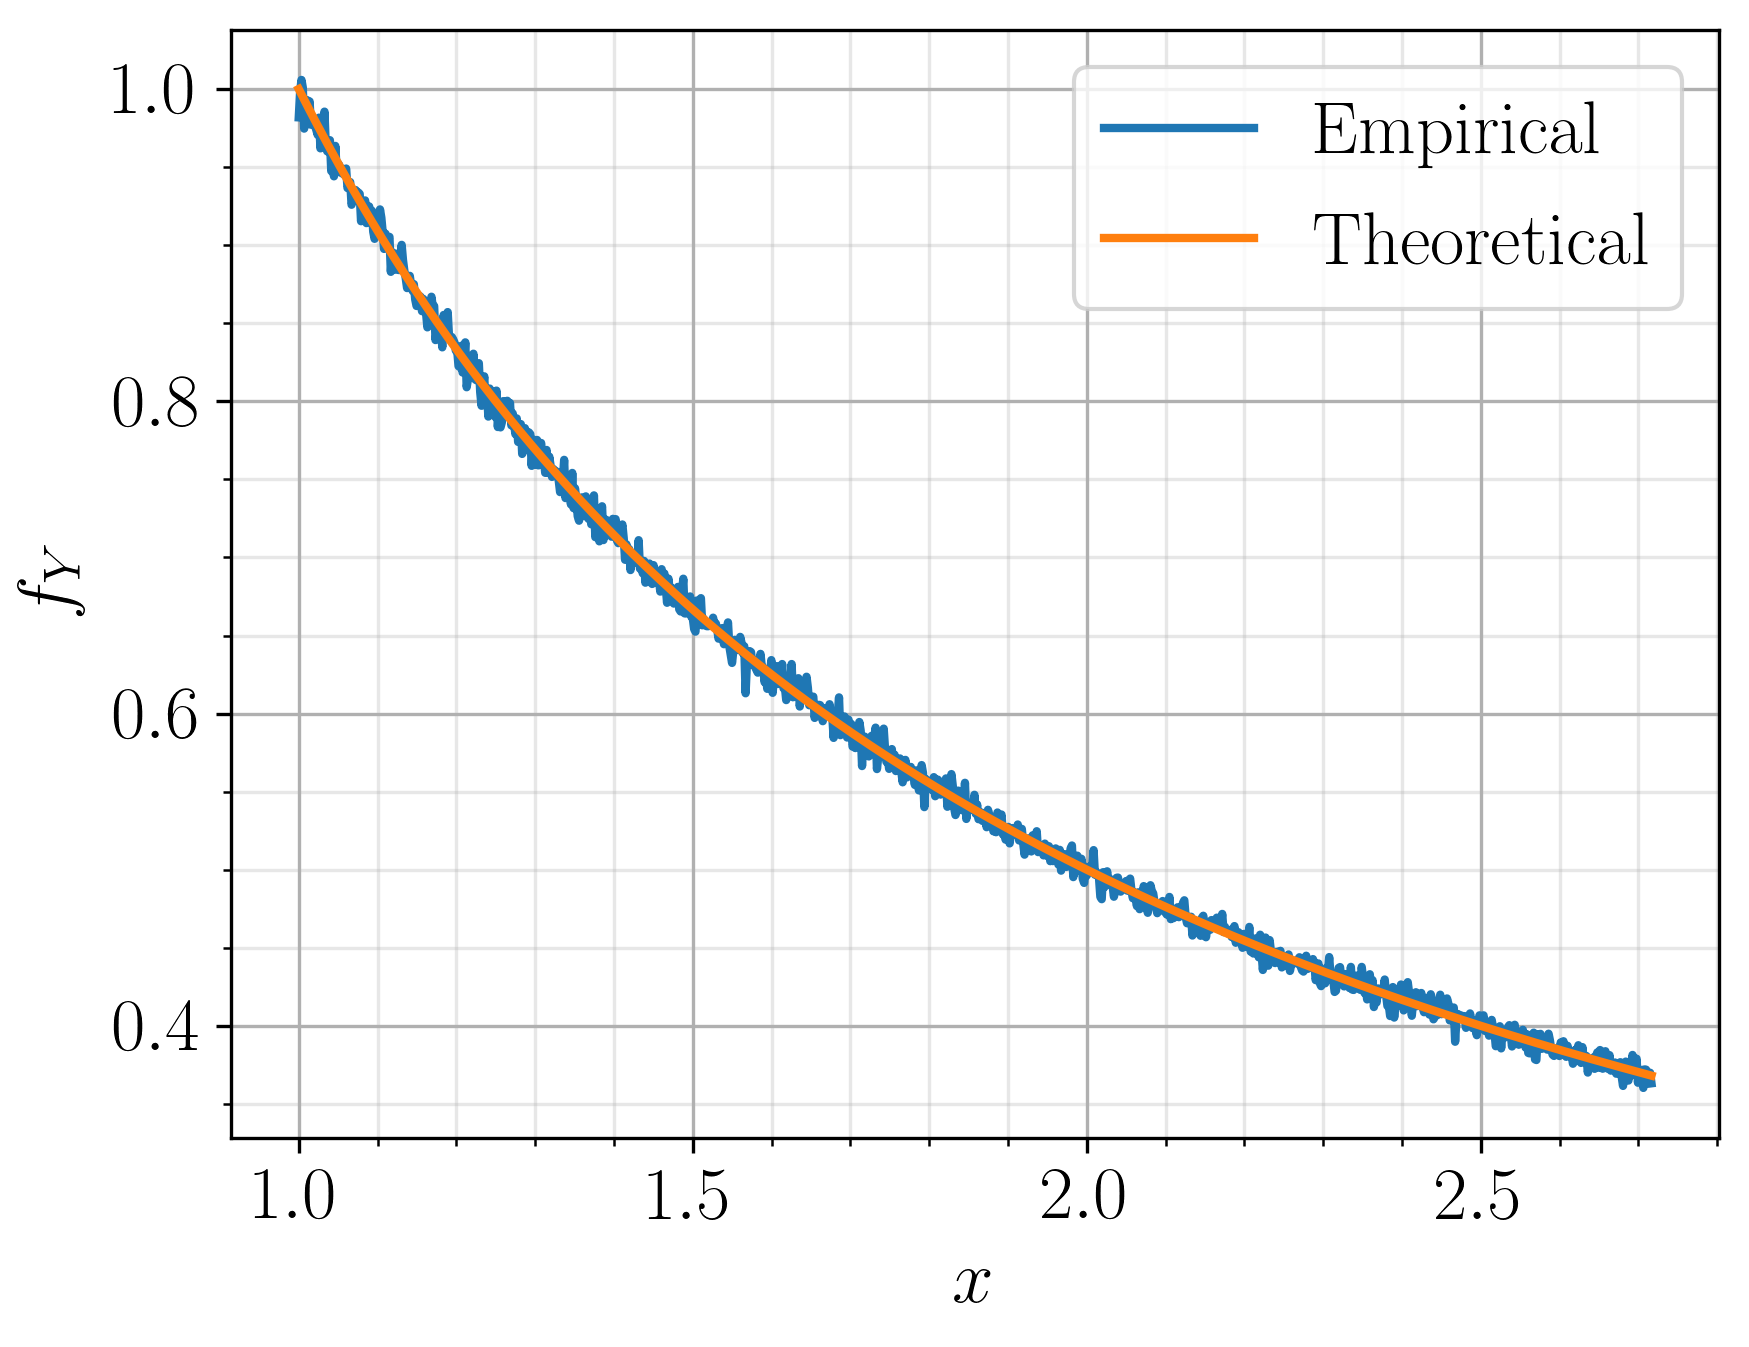
\includegraphics[width=0.8\linewidth]{py/6f.png}
\end{figure}

\section*{Problema 7}
Seja $X$ uma variável aleatória com distribuição uniforme no intervalo $[-1,1)$. Seja ainda $Y =
X^2$.
\begin{align*}
    f_X(x) &= \frac{1}{a}, \; -1 \le x < 1 \qquad \int_{-1}^1 \frac{1}{a} dx = \frac{x}{a}
\bigg\rvert_{-1}^{1} = \frac{2}{a}, \; a = 2\\
    f_X(x) &=
    \begin{cases}
        \frac{1}{2}, \text{ se } -1 \le x < 1 \\
        0, \text{ c.c}
    \end{cases}
\end{align*}
\paragraph*{A.} Calcule a função densidade de probabilidade (PDF) de $Y$
\begin{align*}
    g(x) &= x^2 \qquad g^{-1}(x) = \pm \sqrt{y}
    \begin{cases}
        x_1 = \sqrt{y} \\
        x_2 = -\sqrt{y}
    \end{cases} \qquad g'(x) = 2x \\
    f_Y &= \frac{f_X(\sqrt{y})}{|2\sqrt{y}|} + \frac{f_X(-\sqrt{y})}{|-2\sqrt{y}|} = 2 \left[
        \frac{\frac{1}{2}}{2\sqrt{y} }\right] = \frac{1}{2\sqrt{y}}, \; 0 \le y < 1
\end{align*}

\paragraph*{B.} Calcule o valor esperado de $X$
\begin{align*}
    \mathbb{E}[X] &= \int_{-1}^1 x \cdot \frac{1}{2} dx = 0
\end{align*}

\paragraph*{C.} Calcule a variância de $X$
\begin{align*}
    Var[X] &= \int_{-1}^1 (x-0)^2 \cdot \frac{1}{2} dx = \frac{x^3}{6} \bigg\rvert_{-1}^{1} =
    \frac{1}{3}
\end{align*}

\paragraph*{D.} Calcule o valor esperado de $Y$
\begin{align*}
    \mathbb{E}[Y] &= \int_0^1 y \cdot \frac{1}{2\sqrt{y} } dy = \int_{-1}^1 x^2 \cdot \frac{1}{2} dx = \frac{1}{3}
\end{align*}

\paragraph*{E.} Calcule a variância de $Y$
\begin{align*}
    Var[Y] &= \int_0^1 (y-\frac{1}{3})^2 \cdot \frac{1}{\sqrt{y}} dy =
    \frac{\sqrt{y}(9y^2-10y+5)}{45} \bigg\rvert_{0}^{1} = \frac{4}{45} \\
    Var[Y] &= \mathbb{E}[Y^2] - (\mathbb{E}[Y])^2 \\
    \mathbb{E}[Y^2] &= \int_{-1}^1 x^4 \cdot \frac{1}{2} dx = \frac{1}{5} \\
    Var[Y] &= \frac{9}{45} - \frac{5}{45} = \frac{4}{45}
\end{align*}

\paragraph*{F.} Com base no histograma de diversas realizações empíricas de $Y$, obtenha uma PDF
empírica e compare com o resultado do item \textbf{A}
\begin{figure}[H]
    \centering
    \caption{PDF com Observações Empíricas e Valor Teórico para $10^7$ valores de teste}
    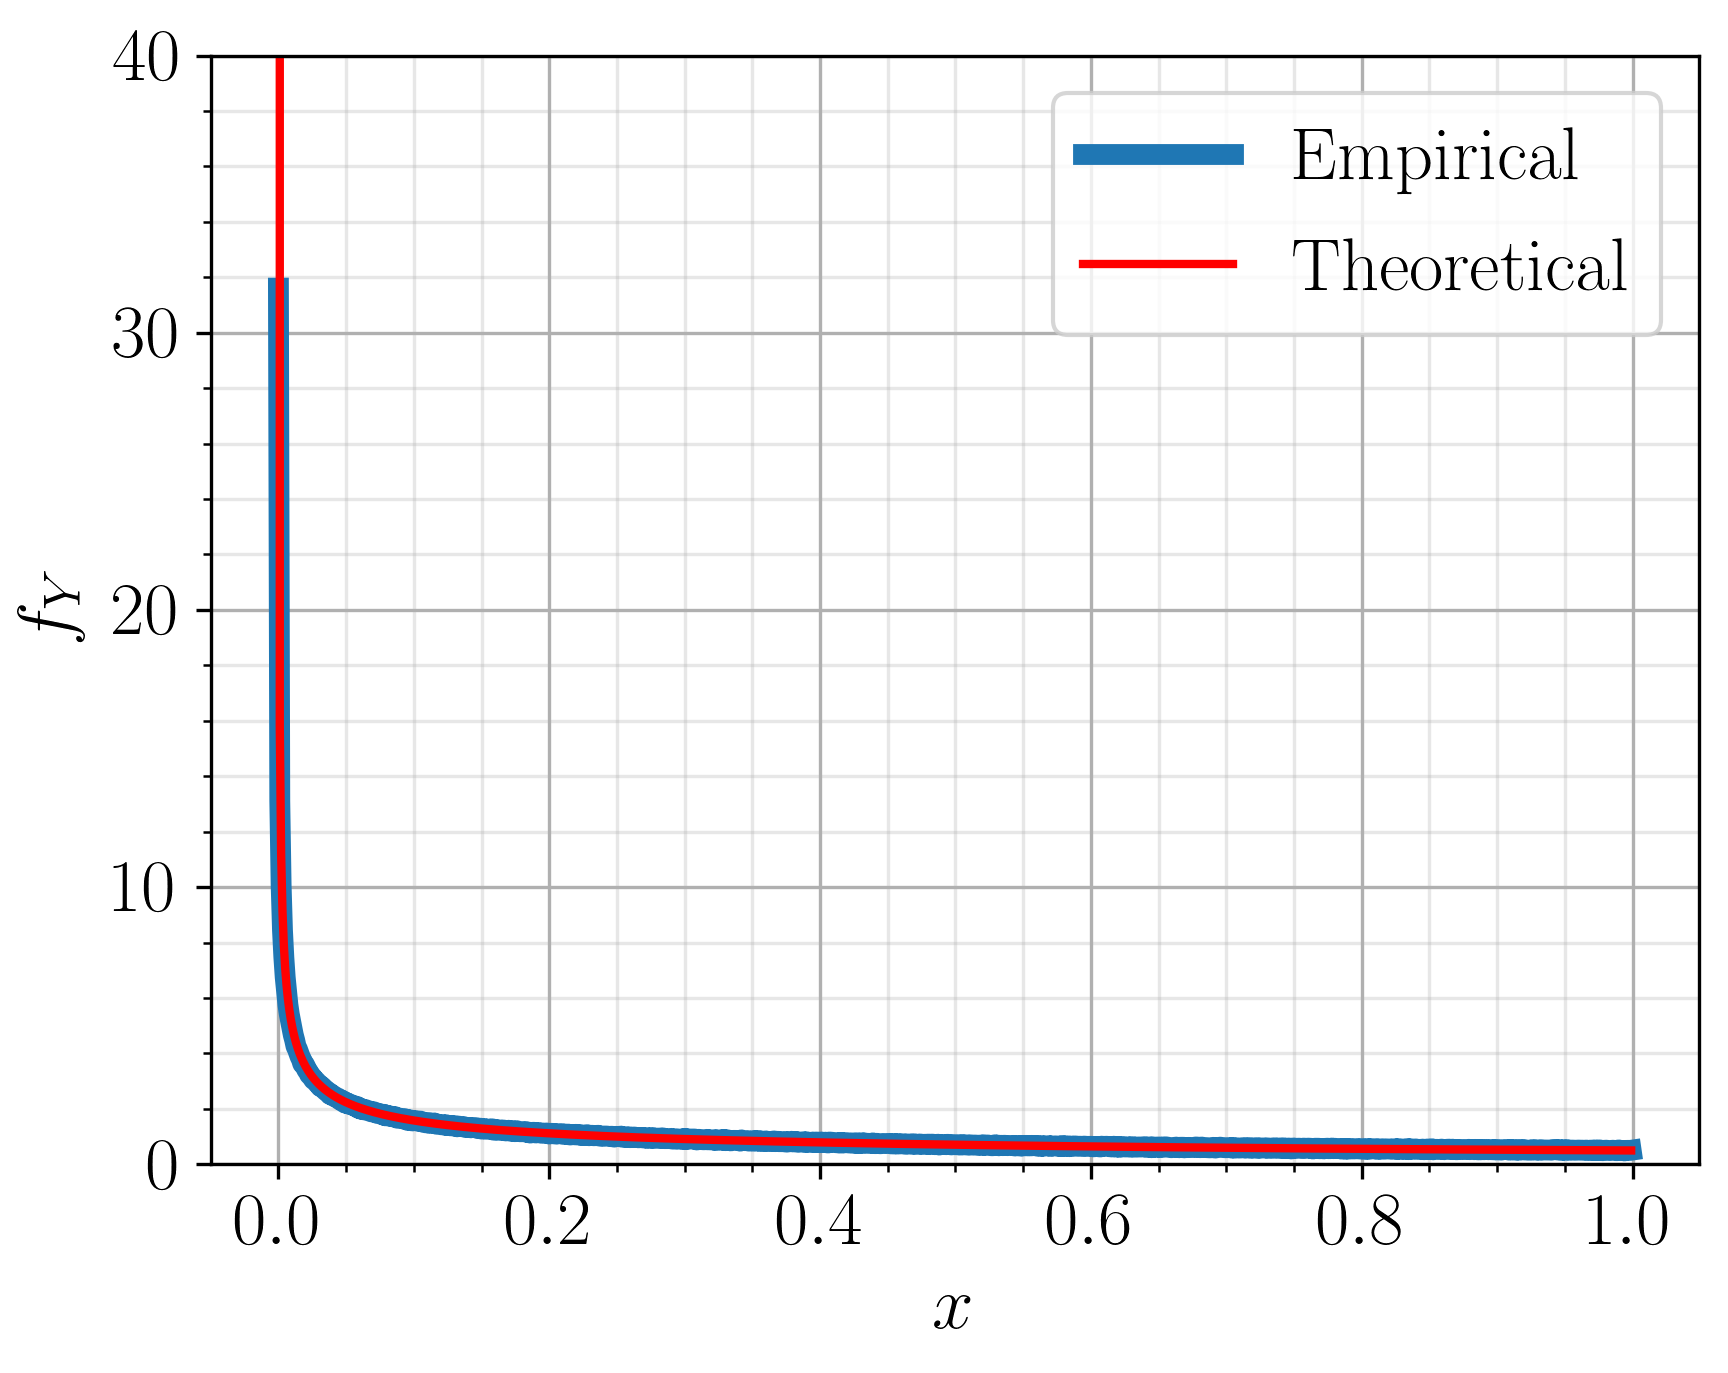
\includegraphics[width=0.8\linewidth]{py/7f.png}
\end{figure}

\section*{Problema 8}
Seja $X$ uma variável aleatória com PDF dada por:
\begin{align*}
    f_X(x) =
    \begin{cases}
        4x^3, \text{ se } 0 < x \le 1 \\
        0, \text{ c.c.}
    \end{cases}
\end{align*}

\paragraph*{A.} Calcule a função densidade de probabilidade (PDF) de $Y$
\begin{align*}
    g(x) &= \sin(\pi x) \qquad g^{-1}(x) =
    \begin{cases}
        x_1 = \frac{\sin^{-1}(y)}{\pi} \\
        x_2 = \frac{\pi - \sin^{-1}(y)}{\pi}
    \end{cases} \qquad g'(x) = \pi \cos(\pi x) \\
    f_Y(y) &= \frac{f_X(\frac{\sin^{-1}(y)}{\pi})}{\pi | \cos(\frac{\pi \sin^{-1}(y)}{\pi}) |} +
    \frac{f_X(\frac{\pi - \sin^{-1}(y)}{\pi})}{\pi | \cos(\frac{\pi - \sin^{-1}(y)}{\pi}) |}
    \qquad \text{ Note que: }
    \begin{cases}
        \cos(\sin^{-1}(\alpha)) = \pm \sqrt{1 - \alpha^2} \\
        \cos(\pi - \beta) = - \cos(\beta)
    \end{cases} \\
    f_Y(y) &= \frac{f_X(\frac{\sin^{-1}(y)}{\pi}) + f_X(\frac{\pi - \sin^{-1}(y)}{\pi})}{\pi
    \sqrt{1 - y^2}}
    = \frac{4 \sin^{-1}(y)^3}{\pi^4 \sqrt{1-y^2}} + \frac{4 \left( \frac{\pi - \sin^{-1}(y)}{\pi}
    \right)^3}{\pi^4 \sqrt{1-y^2}} \\
        f_Y(y) &= \frac{4}{\pi \sqrt{1-y^2}} \left[ \frac{\sin^{-1}(y)}{\pi^3} + \left( \frac{\pi -
        \sin^{-1}(y)}{\pi} \right)^3 \right], \text{ se } 0 \le y < 1, \quad 0 \text{ c.c} \\
\end{align*}%
\begin{align*}
    1 &= \cos(\alpha)^2 + \sin(\alpha)^2 & \cos(\alpha \pm \beta) &= \cos(\alpha)\cos(\beta) \mp
    \sin(\alpha)sen(\beta) \\
    1 &= \cos(\sin^{-1}(\alpha))^2 + \sin(\sin^{-1}(\alpha))^2 & \text{se } \alpha &= \pi, \;
    \cos(\pi)=-1 \; \sin(\pi)=0 \\
    1 &= \cos(\sin^{-1}(\alpha))^2 + \alpha^2 & \cos(\pi - \beta) &= -1 \cos(\beta) + 0\cdot0 \\
    \cos(\sin^{-1}(\alpha)) &= \pm \sqrt{1 - \alpha^2} & \cos(\pi - \beta) &= -\cos(\beta)
\end{align*}

\paragraph*{B.} Calcule o valor esperado de $X$
\begin{align*}
    \mathbb{E}[X] &= \int_0^1 x \cdot 4x^3 dx = \frac{4x^5}{5} \bigg\rvert_{0}^{1} = \frac{4}{5}
\end{align*}
\paragraph*{C.} Calcule a variância de $X$
\begin{align*}
    Var[X] &= \mathbb{E}[X^2] - (\mathbb{E}[X])^2 \\
    \mathbb{E}[X^2] &= \int_0^1 x^2 \cdot 4x^3 dx = \frac{2x^6}{3} \bigg\rvert_{0}^{1} = \frac{2}{3} \\
    Var[X] &= \frac{2}{3} - \frac{16}{25} = \frac{2}{75} \\
\end{align*}

\paragraph*{D.} Calcule o valor esperado de $Y$
\begin{align*}
    \mathbb{E}[Y] &= 4 \int_0^1 x^3 \sin(\pi x) dx \qquad \int u dv = u\cdot v - \int v du \\
    \mathbb{E}[Y] &= 4 \left[ -\frac{x^3 \cos(\pi x)}{\pi} + \frac{3}{\pi} \int_0^1 x^2 \cos(\pi
    x) dx \right] \\
    \mathbb{E}[Y] &= -\frac{4x^3 \cos(\pi x)}{\pi} + \frac{12}{\pi} \left[ \frac{x^2 \sin(\pi
    x)}{\pi} -\frac{2}{\pi} \int_0^1 x \sin(\pi x)dx \right] \\
    \mathbb{E}[Y] &= -\frac{4x^3 \cos(\pi x)}{\pi} + \frac{12x^2 \sin(\pi x)}{\pi^2} -\frac{24
    \sin(pi x)}{\pi^4} + \frac{24 \pi x \cos(pi x)}{\pi^4} \bigg\rvert_{0}^{1} \\
    \mathbb{E}[Y] &= \frac{-4 \pi x(\pi^2x^2-6) \cos(\pi x)}{\pi^4} + \frac{12(\pi^2x^2-2)
    \sin(\pi x)}{\pi^4} \bigg\rvert_{0}^{1} \\
    \mathbb{E}[Y] &= \frac{4}{\pi} - \frac{24}{\pi^3} = 0.4992
\end{align*}
\paragraph*{E.} Calcule a variância de $Y$
\begin{align*}
    Var[Y] &= \mathbb{E}[Y^2] - (\mathbb{E}[Y])^2 \\
    \mathbb{E}[Y^2] &= \int_0^1 4x^3 \cos(\pi x)^2 dx = 2 \int_0^1 x^3 - x^3 \cos(2 \pi x) dx \\
    \int_0^1 x^3 \cos(2 \pi x) dx &= \frac{x^3 \sin(2 \pi x)}{2 \pi} - \frac{3}{2 \pi} \int_0^1
    x^2 \sin(2 \pi x) dx \\
    \int x^2 \sin(ax) dx &= \frac{1}{a^3} \left(2ax \sin(ax) + 2 \cos(ax) -a^2x^2 \cos(ax)
    \right) \\
    \int_0^1 x^2 \sin(2 \pi x) dx &= \frac{1}{(2 \pi)^3} \left[ 4 \pi x \sin(2 \pi x) +2
    \cos(2\pi x) -4 \pi^2x^2 \cos(2 \pi x) \right] = \frac{-4 \pi^2 - 2}{8 \pi^3} \\
    \mathbb{E}[Y^2] &= \frac{1}{2} - 2 [0 -\frac{3}{2 \pi} \cdot -\frac{1}{2 \pi}] =
    \frac{\pi^2 - 3}{2 \pi^2} \\
    Var[Y] &= \frac{\pi^2 - 3}{2 \pi^2} - \left( \frac{4}{\pi} - \frac{24}{\pi^3} \right)^2 =
    0.0988  \\
\end{align*}

\paragraph*{F.} Com base no histograma de diversas realizações empíricas de $Y$, obtenha uma PDF
empírica e compare com o resultado do item \textbf{A}
\begin{figure}[H]
    \centering
    \caption{PDF com Observações Empíricas e Valor Teórico para $10^7$ valores de teste}
    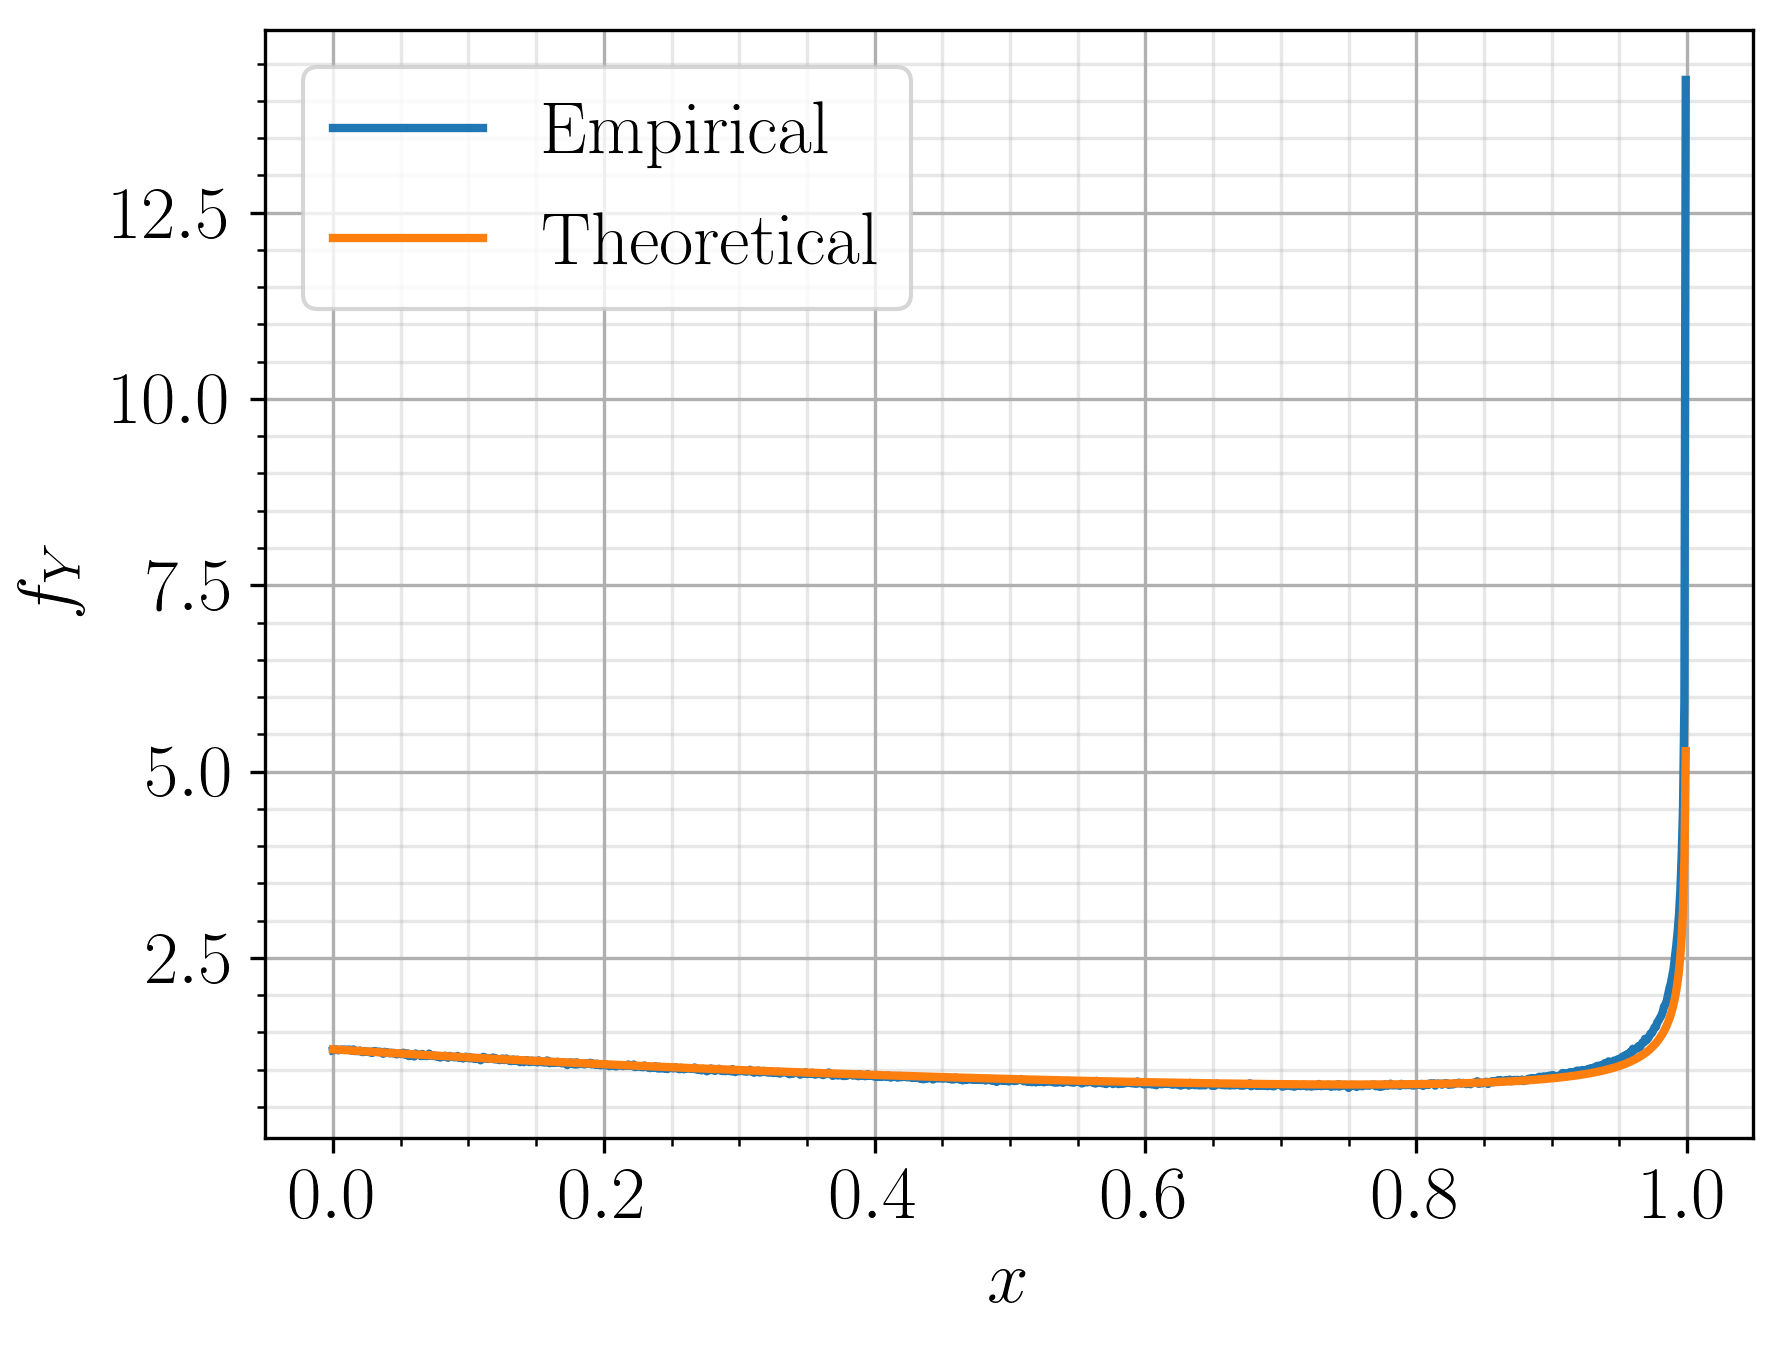
\includegraphics[width=0.8\linewidth]{py/8f.png}
\end{figure}

\section*{Problema 9}
O gráfico a seguir, no qual $M$ é uma constante real, descreve a função densidade de
probabilidade $f_X$ de uma variável aleatória $X$. Acerca de $X$, responda os itens que se
seguem.
\begin{align*}
    f_X(x) &=
    \begin{cases}
        0, \text{ se } x < 0 \\
        Mx, \text{ se } 0 \le x < 1 \\
        -\frac{M}{4}x + \frac{5M}{4}, \text{ se } 1 \le x < 5 \\
        0, \text{ se } x \ge 5
    \end{cases} \\
    1 &= \int_0^1 Mx dx + \int_1^5 -\frac{M}{4}x + \frac{5M}{4} dx, \qquad M = \frac{2}{5} \\
\end{align*}

\paragraph*{A.} Qual o valor esperado de $X$?
\begin{align*}
    \mathbb{E}[X] &= \int_0^5 x f_X(x) dx = 2
\end{align*}

\paragraph*{B.} Qual o momento central de ordem 2 de $X$?
\begin{align*}
    M_C^2[X] &= \mathbb{E}[(X - \mu)^2] = \mathbb{E}[X^2] - (\mathbb{E}[X])^2 = Var[X] \\
    \mathbb{E}[X^2] &= \int_0^5 x^2 f_X(x) dx = \frac{31}{6} \\
    M_C^2[X] &= \frac{31}{6} - 2^2 = \frac{7}{6}
\end{align*}

\paragraph*{C.} Qual o momento central de ordem 3 normalizado de $X$?
\begin{align*}
    Skew[X] &= \widetilde{\mu}_3 = \mathbb{E}\left[ \left( \frac{X - \mu}{\sigma} \right)^3
    \right] = \frac{\mu_3}{\sigma^3} \\
    Skew[X] &= \frac{\mathbb{E}[X^3] -3\mu\mathbb{E}[X^2] +3\mu^2\mathbb{E}[X] -
    \mu^3}{\sigma^3} \\
    Skew[X] &= \frac{\mathbb{E}[X^3] -3\mu(\mathbb{E}[X^2] -\mu\mathbb{E}[X])-\mu^3}{\sigma^3} \\
    Skew[X] &= \frac{\mathbb{E}[X^3] -3\mu\sigma^2 -\mu^3}{\sigma^3} \\
    \mathbb{E}[X^3] &= \int_0^5 x^3 f_X(x) dx = \frac{78}{5} \qquad \mu = 2 \qquad \sigma =
    \sqrt{\frac{7}{6}} \\
    Skew[X] &= \frac{18\sqrt{42}}{245} = 0.4761
\end{align*}

\paragraph*{D.} Qual o momento central de ordem 4 normalizado de $X$?
\begin{align*}
    Kurt[X] &= \mathbb{E}\left[ \left( \frac{X - \mu}{\sigma} \right)^4
    \right] = \frac{\mu_4}{\sigma^4} = \frac{E[(X-\mu)^4]}{(E[(X-\mu)^2])^2} \\
        Kurt[X] &= \frac{\frac{49}{15}}{(\frac{7}{6})^2} = \frac{12}{5} = 2.4 \\
\end{align*}

\paragraph*{E.} Qual a probabilidade de que $X$ seja 3?
0.

\paragraph*{F.} Qual a probabilidade de $X$ esteja no intervalo $[2,4]$?
\begin{align*}
    P_X([2,4]) &= F_X(4) - F_X(2) = \int_2^4 f_X(x)dx = \frac{2}{5} = 0.4 \\
\end{align*}

\paragraph*{G.} Qual a probabilidade de $X$ esteja no intervalo $[2,5]$?
\begin{align*}
    P_X([2,5]) &= F_X(5) - F_X(2) = \int_2^5 f_X(x)dx = \frac{9}{20} = 0.45 \\
\end{align*}

\paragraph*{H.} Qual a probabilidade de que $X$ esteja no intervalo $[2,6]$?
Igual a do item anterior.
\\
\textit{That's all Folks}

\end{document}
